\documentclass[12pt,a4paper,english]{article}
\usepackage[utf8x]{inputenc}
\usepackage{amsmath}
\usepackage{amsthm}
\usepackage{multirow}
\usepackage{listings}
\usepackage[pdftex,usenames,dvipsnames]{color}
\usepackage{graphicx}
\usepackage[pdftex,bookmarks,colorlinks,urlcolor=blue,linkcolor=BlueViolet]{hyperref}  % sollte immer als letztes inkludiert werden

\lstset{numbers=left, numberstyle=\tiny, keywordstyle=\color{blue}, 
numbersep=15pt, language=SQL, basicstyle=\footnotesize, breaklines=true,
showstringspaces=false,tabsize=4}

% Dokumentinfo
\title{Neue Informationssysteme 706.002\\}
\date{\today}
\author{Michael Hraschan, 0831401 \\
				Achleitner Florian, 0830434\\
				Matthias Viertler, 0830605 \\}

\begin{document}

\maketitle

\newpage
%
\tableofcontents % if you want
\clearpage
%

\section{README}
This Assignment is designed to run with php5 and should run flawlessly on xampp 1.7.3.
To get started open ./html/index.html.
It points you to:
\begin{itemize}
	\item The example PHP scripts described in section \ref{sec:php}.
	\item The insert-form and php script described in section \ref{sec:insert}.
	\item The XSL Demo described in section \ref{sec:xsl}.
\end{itemize}

\section{Database schema}

\begin{figure}[htbp]
	\centering
		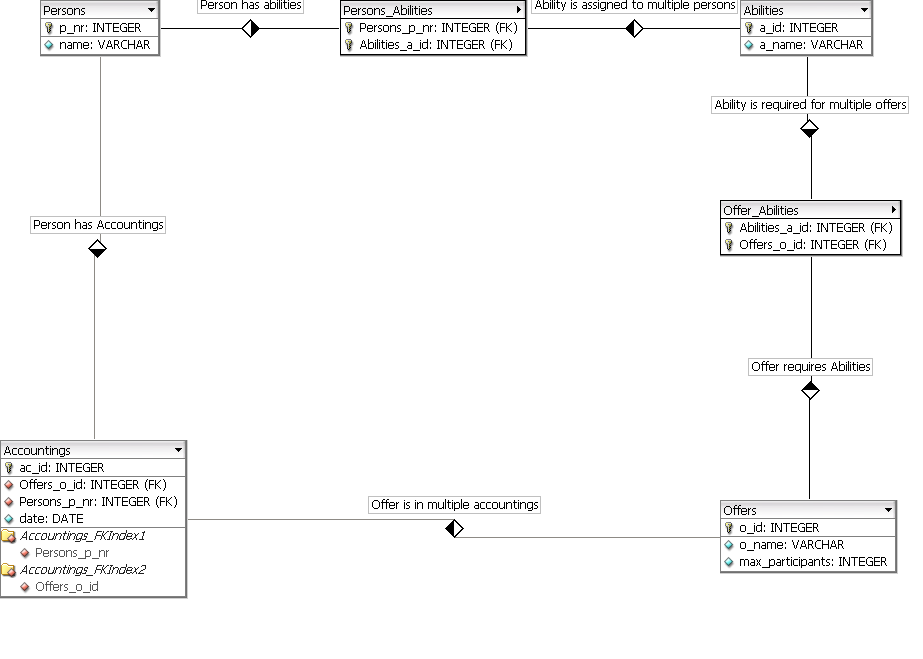
\includegraphics[width=1.00\textwidth]{Images/database_design.png}
	\caption{Scheme of the used database.}
	\label{fig:database_design}
\end{figure}

\begin{itemize}
	\item Domains
		\begin{itemize}
			\item \textbf{p\_nr Integer;} Person number
			\item \textbf{name String;} Person name
			\item \textbf{a\_id Integer;} Ability id
			\item \textbf{a\_name String;} Ability name
			\item \textbf{o\_id Integer;} Offer id
			\item \textbf{o\_name String;} Offer name
			\item \textbf{max\_participants Integer;} Maximal participants for an offer
			\item \textbf{ac\_id Integer;} Accounting id
			\item \textbf{date Date;} Date of the accounting
		\end{itemize}
	\item Relation: Persons(\textbf{\underline{p\_nr}}, name)
	\item Relation: Persons\_Abilities(\textbf{\underline{Persons\_p\_nr, Abilities\_a\_id}})
	\item Relation: Abilities(\textbf{\underline{a\_id}}, a\_name)
	\item Relation: Offer\_Abilities(\textbf{\underline{Abilities\_a\_id, Offers\_o\_id}})
	\item Relation: Offers(\textbf{\underline{o\_id}}, o\_name, max\_participants)
	\item Relation: Accountings(\textbf{\underline{ac\_id}}, date)
\end{itemize}
Two compound primary keys are used.

\subsection{Normal form}
\subsubsection{1. normal form}
The table is in the 1. normal form because each table represents a relation and has no repeating groups. 

\subsubsection{2. normal form}
The table is in the 2. normal form because no non-prime attribute in the tables are funcionally dependent on a part of a candidate key. 

\subsubsection{3. normal form}
The table is in the 3. normal form because every non-prime attribute is non-transitively dependent on every key of the tables.


\section{Practical implementation of the database with mySQL}
\subsection{Creating the user and the database}
Initially we create a user and a database and grant all privileges on that database
to the user.
\begin{lstlisting}
CREATE DATABASE nis;
CREATE USER nis;
GRANT ALL PRIVILEGES ON nis.* TO nis;
\end{lstlisting}

\subsection{Creating the Schema}
These queries generate the tables in the current database.
\lstinputlisting[caption={Creating the tables. (./database/tables.sql)},label=tables.sql]{../database/tables.sql}

\subsection{Inserting initial data}
Insert some sample data into the above created tables.
\lstinputlisting[caption={Inserting initial data. (./database/values.sql)},label=values.sql]{../database/values.sql}

\section{Inserting Test Data with PHP and HTML} \label{sec:insert}
This html/php page allows to insert new persons, new abilities and new links between persons and abilities.
Those are stored in the table \emph{Persons\_Abilities} as described above. Both columns are foreign keys.
The \emph{referential integrity} with the tables Persons and Ablilities must be ensured, i.e. the foreign keys
must exist as primary keys in their parent table. See line 104 in listing \ref{insert.php}.

\lstset{language=HTML}
\lstinputlisting[caption={Inserting data and referential integrity checks in php},label=insert.php]{../php/insert.php}

\section{PHP Scripts and Queries} \label{sec:php}

\lstinputlisting[caption={index.php}]{../php/index.php}


\section{XML Transformation with XSLT} \label{sec:xsl}
XSL - the eXtensible Stylsheet Language - describes how to translate an XML document into another.
Often into HTML. In this example we use an XSL file that translates an XML file containing data
from a database query to HTML.

\subsection{Client-Side Transformation}
This concept sends the XML file to the browser, and adds a line telling the browser about
the XSL stylesheet to use.
\begin{lstlisting}[language=XML]
<?xml-stylesheet type="text/xsl" href="../xsl/transform.xsl"?>
\end{lstlisting}
The MIME type in the HTTP header needs to be set to text/xml in PHP. 
\begin{lstlisting}[language=PHP]
header('Content-Type: text/xml');
\end{lstlisting}

Then browser
interprets the XML file and transforms it according to the XSL file

\subsection{Server-Side Transformation}
This variant uses the PHP component \emph{XsltProcessor} to convert the XML to HTML
and send the result to the browser.

\subsection{Listings}
The php script uses client-side transformation if the query string passes serverclient=client.
\lstinputlisting[caption={XSL tranformation php script. (./php/create\_xml.php)},language=PHP]{../php/create_xml.php}
\lstinputlisting[caption={The XSL file. (./xsl/transform.xsl)},language=XML]{../xsl/transform.xsl}




\end{document}
